% Fig. 5  Round 7 ablation (single column, 3.45 in). Data: ../data/round7_ablation.csv,
% from research_improvement/03_ablation_results.csv (frozen build 38b60d1). Generated by ../make_r7_figures.py.
\documentclass[border=2pt]{standalone}
% Shared settings for all InsightFlow AI figures (Times, grayscale, sized for IEEE print).
\usepackage[T1]{fontenc}
\usepackage{mathptmx}
\usepackage{tikz}
\usetikzlibrary{positioning,arrows.meta,calc,fit,patterns,shapes.geometric}
\tikzset{
  >={Stealth[length=4pt,width=3.5pt]},
  stage/.style={draw,rounded corners=1.5pt,fill=gray!8,align=center,inner sep=2.5pt,font=\fontsize{7.5}{8.6}\selectfont},
  ext/.style={draw,dashed,rounded corners=1.5pt,align=center,inner sep=2.5pt,font=\fontsize{7.5}{8.6}\selectfont},
  note/.style={align=left,font=\fontsize{7}{8}\selectfont},
  flow/.style={->,thick},
  dflow/.style={->,dashed},
  every node/.append style={execute at begin node={\hyphenpenalty=10000\exhyphenpenalty=10000}},
}

\usepackage{pgfplots}
\pgfplotsset{compat=1.17}
\begin{document}
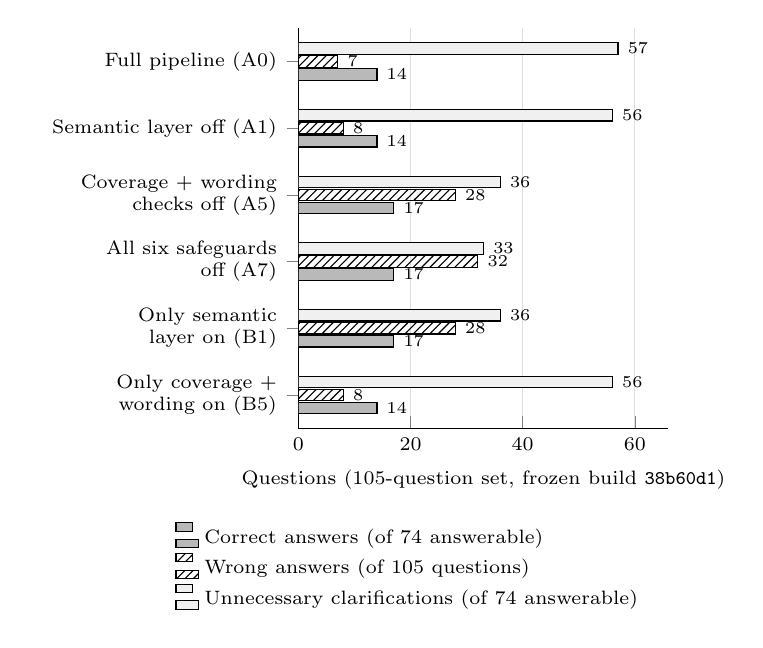
\begin{tikzpicture}
\begin{axis}[
  width=1.85in, height=2.0in, scale only axis=true,
  xbar=0.5pt, bar width=4.2pt, xmin=0, xmax=66,
  xlabel={Questions (105-question set, frozen build \texttt{38b60d1})},
  xlabel style={font=\fontsize{7.5}{8.6}\selectfont},
  ytick=data, y dir=reverse, symbolic y coords={A0,A1,A5,A7,B1,B5},
  yticklabels={{Full pipeline (A0)},{Semantic layer off (A1)},{Coverage + wording checks off (A5)},{All six safeguards off (A7)},{Only semantic layer on (B1)},{Only coverage + wording on (B5)}},
  yticklabel style={align=right,font=\fontsize{7}{8}\selectfont,text width=1.2in},
  xticklabel style={font=\fontsize{7.5}{8.6}\selectfont},
  enlarge y limits=0.1, axis x line*=bottom, axis y line*=left, xmajorgrids, grid style={gray!25},
  nodes near coords, nodes near coords style={font=\fontsize{6.5}{7.5}\selectfont,anchor=west},
  point meta=explicit symbolic,
  legend style={font=\fontsize{7}{8}\selectfont,at={(0.3,-0.22)},anchor=north,legend columns=1,draw=none,cells={anchor=west}},
]
\addplot[draw=black,fill=gray!55] coordinates {(14,A0)[14] (14,A1)[14] (17,A5)[17] (17,A7)[17] (17,B1)[17] (14,B5)[14]};
\addplot[draw=black,pattern=north east lines] coordinates {(7,A0)[7] (8,A1)[8] (28,A5)[28] (32,A7)[32] (28,B1)[28] (8,B5)[8]};
\addplot[draw=black,fill=gray!12] coordinates {(57,A0)[57] (56,A1)[56] (36,A5)[36] (33,A7)[33] (36,B1)[36] (56,B5)[56]};
\legend{{Correct answers (of 74 answerable)},{Wrong answers (of 105 questions)},{Unnecessary clarifications (of 74 answerable)}}
\end{axis}
\end{tikzpicture}
\end{document}
